\documentclass[11pt,a4paper]{article}
\usepackage[T1]{fontenc}
\usepackage{lmodern}
\usepackage[margin=24mm,headheight=15pt]{geometry}
\usepackage{amsmath,amssymb,mathtools}
\usepackage{graphicx,booktabs,tabularx,longtable,array}
\usepackage[dvipsnames]{xcolor}
\usepackage{tikz}
\usetikzlibrary{arrows.meta,positioning,fit,backgrounds,calc}
\usepackage[most]{tcolorbox}
\usepackage{enumitem,microtype,fancyhdr,titlesec}
\usepackage[hyphens]{url}
\usepackage[colorlinks=true,linkcolor=RoyalBlue,citecolor=RoyalBlue,urlcolor=RoyalBlue,
 pdftitle={Understanding Our SuperMimic Implementation},
 pdfauthor={IsaacLab SuperMimic project},bookmarksnumbered=true]{hyperref}
\definecolor{ink}{HTML}{14263D}
\definecolor{blue}{HTML}{2563EB}
\definecolor{orange}{HTML}{C65D12}
\definecolor{pale}{HTML}{EFF6FF}
\definecolor{green}{HTML}{0F766E}
\setlength{\parindent}{0pt}
\setlength{\parskip}{0.55em}
\setlength{\emergencystretch}{2em}
\renewcommand{\arraystretch}{1.18}
\setlist{itemsep=0.25em,topsep=0.3em,leftmargin=*}
\setlist[description]{style=nextline,leftmargin=0pt,labelindent=0pt,labelwidth=0pt,labelsep=0pt,font=\bfseries}
\renewcommand{\tabularxcolumn}[1]{>{\raggedright\arraybackslash}p{#1}}
\titleformat{\section}{\Large\bfseries\color{ink}}{\thesection}{0.7em}{}
\titleformat{\subsection}{\large\bfseries\color{ink}}{\thesubsection}{0.7em}{}
\pagestyle{fancy}
\fancyhf{}
\fancyhead[L]{\small\color{ink}SuperMimic on IsaacLab: a practical tutorial}
\fancyfoot[L]{\small\color{gray}Implementation and completed-run snapshot}
\fancyfoot[R]{\thepage}
\renewcommand{\headrulewidth}{0.3pt}
\newtcolorbox{idea}[1]{colback=pale,colframe=blue!65,boxrule=0.5pt,arc=2pt,
 title={#1},fonttitle=\bfseries,breakable,left=9pt,right=9pt,top=6pt,bottom=6pt}
\newtcolorbox{caution}[1]{colback=orange!5,colframe=orange!70,boxrule=0.5pt,arc=2pt,
 title={#1},fonttitle=\bfseries,breakable,left=9pt,right=9pt,top=6pt,bottom=6pt}
\newcommand{\R}{\mathbb{R}}
\newcommand{\E}{\mathbb{E}}
\newcommand{\sg}{\operatorname{stopgrad}}
\newcommand{\clip}{\operatorname{clip}}
\newcommand{\norm}[1]{\left\lVert #1\right\rVert}
\newcommand{\code}[1]{\texttt{\small\detokenize{#1}}}
\newcommand{\src}[1]{\par{\footnotesize\color{gray}\raggedright\ttfamily Implementation: \detokenize{#1}.\par}}
\tikzset{box/.style={draw=blue!60,fill=pale,rounded corners=2pt,align=center,
 minimum height=10mm,font=\small,inner sep=5pt},
 graybox/.style={box,draw=gray!65,fill=gray!7},
 arr/.style={-{Latex[length=2mm]},thick,draw=ink},
 grad/.style={-{Latex[length=2mm]},thick,dashed,draw=orange}}

\begin{document}
\hypersetup{pageanchor=false}
\begin{titlepage}
\vspace*{12mm}
{\color{blue}\large ISAACLAB / G1 MOTION TRACKING}\par
\vspace{8mm}
{\color{ink}\Huge\bfseries Understanding Our\\[3mm] SuperMimic Implementation}\par
\vspace{7mm}
{\Large A tutorial on goal-conditioned policies, learned dynamics,\\[2mm]
 imitation rewards, and training through imagination}\par
\vspace{10mm}
\begin{idea}{Who this document is for}
You know the basic reinforcement-learning loop and the idea of an MDP, but want
to understand exactly what ``goal conditioning,'' a ``world model,'' and
``backpropagation through imagined rollouts'' mean in this project. The discussion
starts with those concepts, then connects every important quantity to the actual
network dimensions and training code.
\end{idea}
\vspace{6mm}
\begin{tabularx}{\linewidth}{@{}lX@{}}
Project & \code{projects/supermimic}, branch \code{milad/supermimic}\\
Robot / simulator & Unitree G1, 29 actuated joints; IsaacLab + Newton/MJWarp\\
Training data & 40 G1-retargeted LAFAN1 clips, approximately 2.45 hours\\
Completed run & 320,000 simulator iterations; approximately 21 hours 26 minutes\\
Final evaluation & 0.9349 normalized return; 0/40 failed five-second windows\\
Document date & November 6, 2026, Pacific time\\
\end{tabularx}
\vfill
{\small This describes our implemented experiment, verified against its source
and saved outputs. It is an explanatory implementation report, not the authors'
official documentation or a claim of an exact reproduction of every paper setting.
The published SuperMimic paper and project are credited in the references.}
\end{titlepage}
\hypersetup{pageanchor=true}

\tableofcontents
\clearpage

\section*{How to read this tutorial}
\addcontentsline{toc}{section}{How to read this tutorial}
The main conceptual path is Sections~\ref{sec:overview}--\ref{sec:goals}, followed
by the network discussion in Section~\ref{sec:networks} and the training explanation
in Sections~\ref{sec:loop}--\ref{sec:critic}. The remaining sections make the
implementation precise and explain the evidence from the completed run.

There are three kinds of statements throughout the document:
\begin{itemize}
\item \textbf{Concepts}: explanations of control, conditioning, gradients, and value
functions that do not depend on our particular layer widths.
\item \textbf{Implementation facts}: the actual tensors, equations, simulator settings,
and optimizer schedule in our checkout. Source pointers identify their owners.
\item \textbf{Measured results}: values from the saved readiness report, final metrics,
or the 40-video batch. Each result is tied to its evaluation protocol.
\end{itemize}
The notation is introduced where it is used and collected in
Appendix~\ref{app:notation}. A tensor-dimension worksheet and source-reading guide
are in Appendices~\ref{app:dimensions} and~\ref{app:source}.

\begin{idea}{The explanation in one paragraph}
We provide the robot with a desired future motion and its recent sensor history.
A shared policy chooses joint-position commands. Physics determines what actually
happens, and those real transitions train a neural dynamics model. We then use
that model to imagine short futures, score them against the desired motion, and
differentiate the score back into the policy. A value network estimates what
happens beyond the short imagined horizon. The desired motion tells the system
\emph{what to achieve}; the learned policy discovers \emph{how to achieve it under physics}.
\end{idea}

\section{The complete system before the details}\label{sec:overview}
\subsection{What task are we solving?}
Our robot is a floating-base humanoid. Its feet may touch, slide on, or leave the
floor; it can fall; and its motors have limited effort. We want it to follow a
time-indexed reference motion: the intended body pose, joint motion, orientation,
and velocities at each instant. The reference might describe walking, dancing,
running, or lying down and getting up.

This is a \textbf{motion tracker}. It is not currently a system that receives a
sentence such as ``walk to the door,'' generates a new motion plan, or chooses
which skill to perform. A reference clip and its current frame already exist.
The controller learns to track them in closed loop.

SuperMimic motivates learning a differentiable dynamics model alongside a
reference-conditioned policy, using short imagined rollouts for policy
optimization~\cite{supermimic}. Our implementation follows that central idea,
while making its own explicit choices about state representation, normalization,
actuation, and experiment scale.

\subsection{One control step: what those diagram labels actually mean}\label{sec:plainstep}
Assume we have selected a walking clip and the robot is currently partway through
it. We need a command for the next 20 milliseconds. There are two different
sources of information: \emph{the reference file describes the motion we want},
and \emph{the robot's observations describe the motion actually happening}.

\paragraph{1. Read the desired motion: ``future-reference features.''}
We look up the reference at the current time and at 0.1, 0.2, through 0.9 seconds
ahead. A reference is a stored target trajectory. For example, one joint channel
could request the following illustrative values:
\begin{center}
\begin{tabular}{@{}lrrr@{}}
\toprule
Time relative to now & 0.0 s & 0.1 s & 0.2 s\\
\midrule
Desired left-knee angle & 0.60 rad & 0.65 rad & 0.70 rad\\
\bottomrule
\end{tabular}
\end{center}
The actual feature vector contains all 29 target joint angles, all 29 target
joint velocities, and six numbers describing desired root orientation relative
to the current robot, at each of ten reference times. That is
$(29+29+6)\times10=640$ numbers. ``Features'' just means this selected numerical
description. The function \code{goal()} assembles it from stored data and the
current orientation; no neural network is needed for that assembly.
These are \textbf{desired future states}, available because we already have the
clip. They are distinct from a world model's predictions of what the robot
will actually do after a command.

\paragraph{2. Summarize the desired motion: the ``motion encoder.''}
A neural network reads those 640 numbers and produces 32 numbers. This is the
motion encoder. Its job is to retain information useful for choosing commands,
such as patterns in the requested upcoming joint movement. The meanings of the
32 coordinates are learned; we do not assign a coordinate the name ``walking''
or ``knee speed.'' One shared encoder is used for every reference clip.

\paragraph{3. Read what the robot is actually doing.}
Independently, we assemble ten recent sensor observations: joint angles and
velocities, base angular velocity, gravity direction, and previous commands.
There are 930 numbers. In the illustrative knee example, the actual knee might
currently be at 0.50 rad even though the reference requests 0.60 rad. A feedback
controller needs this actual condition as well as the desired motion.

\paragraph{4. Choose a coordinated command: the ``action decoder.''}
A second neural network reads the 930 observation-history values together with
the encoder's 32 values. From those $930+32=962$ inputs it produces 29 normalized
joint-setpoint commands. This is the action decoder. Here ``decoder'' means a
learned controller producing actions; it does not reconstruct the original
640-number reference vector. Its output is also not simply the desired joint
angle minus the observed angle. It learns coordinated commands for all 29
joints under balance, contact, actuator, and tracking requirements.

\paragraph{5. Execute, observe, and repeat.}
An explicit scale and default-pose offset convert the 29 outputs to joint-position
targets for the drives. Physics advances 20 milliseconds. The robot is observed
again, the reference advances one frame, and all these steps repeat. We do not
assume the last command achieved the requested pose.

\begin{idea}{A plain-language reading of the pipeline}
\textbf{Future-reference features:} numbers describing what motion we want.\\
\textbf{Motion encoder:} learned compression of that desired motion.\\
\textbf{Action decoder:} a learned controller using the compressed target and
recent robot measurements to choose joint commands.\\
\textbf{Encoder plus decoder:} the policy. Training adjusts both networks
together to improve tracking return; executing a new reference uses the same
trained weights with new inputs.
\end{idea}

\subsection{Three learned components, with different jobs}
\begin{tabularx}{\linewidth}{@{}lXX@{}}
\toprule
Component & Question answered & How it learns\\
\midrule
Policy / actor $\pi_\theta$ & Given my recent observations and desired motion,
what action should I take? & Maximize imagined tracking return.\\
World model $F_\phi$ & Given a physical state and action, what will the next
physical state be? & Fit transitions collected from physics.\\
Critic $V_\psi$ & Given this state and desired motion, how much future tracking
reward can the current controller expect? & Regress to imagined lambda returns.\\
\bottomrule
\end{tabularx}
The parameters $\theta$, $\phi$, and $\psi$ are separate sets of neural-network
weights. The policy itself contains both a motion encoder and an action decoder;
they are trained together by the same policy objective.

\begin{figure}[htbp]
\centering
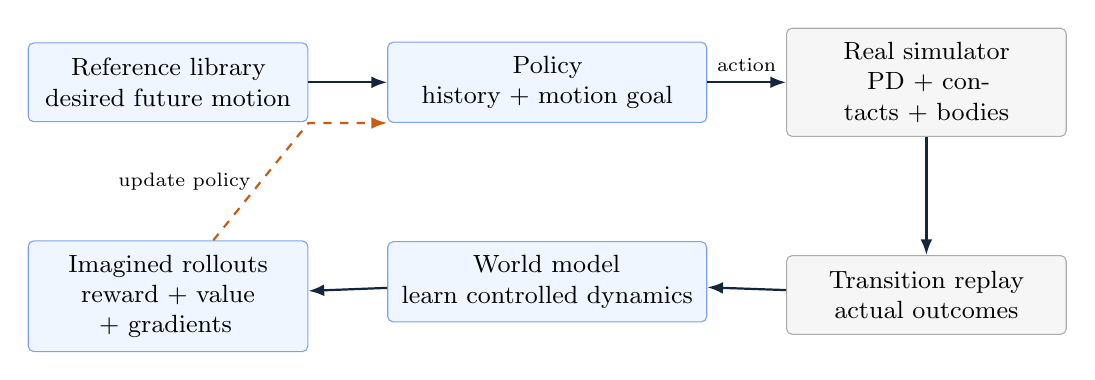
\begin{tikzpicture}[node distance=9mm and 10mm]
\node[box,text width=32mm] (ref) {Reference library\\desired future motion};
\node[box,text width=37mm,right=of ref] (policy) {Policy\\history + motion goal};
\node[graybox,text width=32mm,right=of policy] (sim) {Real simulator\\PD + contacts + bodies};
\node[graybox,text width=32mm,below=15mm of sim] (replay) {Transition replay\\actual outcomes};
\node[box,text width=37mm,below=15mm of policy] (model) {World model\\learn controlled dynamics};
\node[box,text width=32mm,below=15mm of ref] (imag) {Imagined rollouts\\reward + value + gradients};
\draw[arr] (ref)--(policy);
\draw[arr] (policy)--node[above,font=\scriptsize]{action}(sim);
\draw[arr] (sim)--(replay);
\draw[arr] (replay)--(model);
\draw[arr] (model)--(imag);
\draw[grad] (imag)--node[left,font=\scriptsize]{update policy}(ref.south east |- policy.south) -- (policy.south west);
\end{tikzpicture}
\caption{The simulator supplies evidence. The neural model supplies a differentiable
training path. The dashed arrow represents a policy-parameter update, not a
gradient through the actual simulator. The reference library is fixed.}
\end{figure}

\subsection{What runs when the trained controller is deployed?}
At each control step, construct the observation history and reference goal, run
the encoder and decoder once, and send the resulting command to the joint drives.
The world model and critic are training tools: the runtime policy does not run
32-step optimization or search over candidate action sequences.

\begin{idea}{A useful separation}
The reference is a \emph{description of desired behavior}. The policy is a
\emph{feedback controller}. The world model is a \emph{predictor of physical outcomes}.
The critic is a \emph{predictor of future task success}. These are related, but
none can simply replace the others.
\end{idea}

\section{The MDP, the reference clock, and partial observations}\label{sec:mdp}
\subsection{The physical state is only part of the task state}
Let $x_t$ denote the simulator's full physical state, including any internal
quantities necessary to advance the numerical simulation. The learned model
uses an extracted robot state $s_t$, described in Section~\ref{sec:representations}.
Let $c$ identify the selected motion clip and $k_t$ identify its current reference
frame. Write $\bar s_{c,k}$ for a reference state; the bar means \emph{desired},
not predicted.

The same robot pose can be good for one reference frame and bad for another.
Also, the reward penalizes changing the previous action, and training imposes an
episode timeout. A useful formal task state is therefore
\begin{equation}
z_t=(x_t,c,k_t,a_{t-1},\ell_t),
\end{equation}
where $\ell_t$ is the number of control steps since reset. This makes the desired
motion, action-smoothness context, and timeout state explicit. If we want the
closed-loop system with a finite-history controller to be Markov as well, we can
augment this state with the controller's observation-history buffer.

\begin{caution}{The 71-number vector is an engineering state representation}
It represents the robot's pose and velocities, not every hidden variable inside
the solver or actuator implementation. Treating it as sufficient for a one-step
neural dynamics model is an approximation. That approximation is tested against
simulator transitions; it is not a mathematical guarantee that all numerical
physics history has been captured.
\end{caution}

\subsection{Action, transition, reward, and reset}
The main ingredients can now be specified precisely.
\begin{description}
\item[Action.] $a_t\in[-10,10]^{29}$ is a vector of normalized joint-setpoint
commands. It is converted to position targets and executed by PD-like drives.
It is neither a vector of torques nor a command to teleport joints.
\item[Transition.] Physics advances by four 5~ms steps, giving a 20~ms control
transition. The reference advances independently: $k_{t+1}=k_t+1$.
\item[Reward.] Compare the resulting physical motion against
$\bar s_{c,k_t+1}$, then subtract action-change and joint-limit penalties.
\item[Failure.] Reference-relative root-height or tilt error exceeds a threshold.
\item[Timeout.] The clip ends, or the training episode reaches 500 control steps
(10 seconds). A timeout is kept distinct from tracking failure.
\item[Initial-state distribution.] Select a clip uniformly, select a valid frame
uniformly within that clip, set the robot to its reference state, and add small
joint-position noise during training.
\end{description}
The objective is high expected discounted tracking reward over these clips,
starting states, and training perturbations. This is not a navigation objective
and does not discover its own high-level goals.

\subsection{Why the policy has partial observations}
The actor does not see all of $z_t$ or even all 71 components of $s_t$. Its direct
sensor input contains joints, base angular velocity, gravity direction, and the
previous action. The robot's global position and root linear velocity are absent.
It also receives a motion-goal representation built using the current root
orientation. Thus the control problem is naturally viewed as partially observed.

The ten-frame history gives the feedforward actor temporal information. For
example, similar instantaneous poses can have different recent motion and action
histories. Stacking observations lets an MLP use those differences without an RNN.
It does not prove that every hidden quantity can be reconstructed.

The critic receives richer physical-state features than the actor's direct
sensor stream. This is a form of \textbf{asymmetric actor--critic information}:
training can use information that is unavailable to the direct runtime sensor
input. We must still account for the orientation estimate needed by the goal
constructor before claiming hardware compatibility.
\src{environment.py: TrackingEnv.read/reset/step; task.py: observation/termination; train.py: evaluate}

\section{Goal conditioning, from intuition to exact tensors}\label{sec:goals}
\subsection{Why an unconditional policy is ambiguous}
Imagine the robot is standing still. You might want it to begin walking, crouch,
raise an arm, or start a dance. Its current physical state alone does not tell us
which action is desired. An unconditional deterministic policy $a=\pi_\theta(h)$,
where $h$ is recent sensor history, must produce the same action for the same
history. It cannot respond differently to two unobserved requests.

With a goal input, the policy becomes
\begin{equation}\label{eq:conditioned}
a_t=\pi_\theta(h_t,g_t).
\end{equation}
$h_t$ tells the policy \emph{what is happening}; $g_t$ tells it \emph{what should
happen}. We can hold $h_t$ fixed and change $g_t$, obtaining a different action
from the same network weights.

\begin{idea}{Conditioning changes the input, not the identity of the network}
There is one shared set of weights. It is not one network per clip, a lookup
table of trained skills, or an online weight update every time we change motion.
Conditioning means making the action a function of an additional input.
\end{idea}

This is closely analogous to a thermostat using both measured temperature and a
desired setpoint. The difference is scale: our desired setpoint is a sequence of
future joint and orientation targets, and the controller is learned under
nonlinear floating-base contact dynamics.

\subsection{A goal need not be a single final destination}
In goal-conditioned navigation, $g$ might be a desired position. In our motion
tracker, it is a \textbf{short future reference trajectory}. Calling it a goal
does not imply a sparse terminal reward, a terminal-only objective, or a goal that
remains constant for the episode.

At reference frame $k$, the policy gets samples at
\begin{equation}
k,\ k+5,\ k+10,\ldots,k+45.
\end{equation}
At 50~Hz, their times are $0,0.1,\ldots,0.9$ seconds ahead. This preview is useful:
a controller can begin shifting weight before a future step or lean in
anticipation of a rapid upper-body movement. A single current-pose target cannot
express as much of that intended future.

The reference clock is externally advanced by one frame per action. The policy
does not choose how quickly the clip plays or learn a separate phase controller.
Future sampling clamps at the final frame of the selected clip.

\subsection{The exact 640-dimensional goal}
Let $q_t\in\R^{29}$ denote robot joint positions, and $Q_t$ its root quaternion.
For future sample $i\in\{0,\ldots,9\}$ define
\begin{align}
Q^{\mathrm{rel}}_{t,i}&=Q_t^{-1}\otimes\bar Q_{c,k_t+5i},\\
b_{t,i}&=\left[
\bar q_{c,k_t+5i},\ \dot{\bar q}_{c,k_t+5i},\
R(Q^{\mathrm{rel}}_{t,i})e_x,\ R(Q^{\mathrm{rel}}_{t,i})e_y
\right],\\
g_t&=\operatorname{concat}_{i=0}^{9} b_{t,i}\in\R^{640}.
\end{align}
Here $\otimes$ is quaternion composition, $R(Q)$ converts a quaternion to a
rotation, and $e_x,e_y$ are unit basis vectors. Each sample has
$29+29+3+3=64$ numbers. Two rotated basis vectors provide six continuous rotation
features; a valid third axis can be recovered from their cross product.

Reference joint angles and velocities are absolute target joint quantities in
this representation, not already-computed joint errors. The decoder can compare
them with the observed joints. Reference root orientation is expressed relative
to the current robot orientation, giving an explicit orientation discrepancy.

\begin{caution}{The goal does not contain everything in the reference file}
It contains no reference root position or root linear velocity. Those quantities
are available to the training reward and physical-state-based calculations.
The actor therefore has no direct global-position-error measurement with which
to correct arbitrary accumulated world-position drift. A high tracking score
under our reset and evaluation conditions does not remove this information limit.
\end{caution}

\begin{figure}[htbp]
\centering
\includegraphics[width=\linewidth]{figures/goal_preview.pdf}
\caption{Actual reference left-knee signals from two clips, each starting at
reference frame 250. Dots mark the ten samples used in a goal. Only one of the
29 joint-position channels is shown; joint velocities and relative root
orientations are also supplied. These are reference signals, not policy actions
or a claimed rollout comparison.}
\end{figure}

\subsection{The goal changes as the robot changes}
The joint targets are fixed data for a selected clip and frame. However, the
relative-orientation part depends on the \emph{current} robot orientation. If the
robot rotates unexpectedly, that part changes even at the same reference frame.

This also matters in imagination: after the model predicts a new robot state,
the next goal is recomputed from that predicted state and the next reference
preview. Gradients can therefore pass through the state-dependent goal
construction. The reference values themselves are constants; they are not
optimized to make the task easier.

\subsection{How conditioning changes the actor and critic}
Our actor factors Equation~\eqref{eq:conditioned} into an encoder and decoder:
\begin{align}\label{eq:encoder}
u_t&=\tanh\!\left(E_\theta(N_g(g_t))\right)\in[-1,1]^{32},\\
a_t&=\clip\!\left(D_\theta([\operatorname{flatten}(N_o(h_t)),u_t]),-10,10\right).
\end{align}
$N_g$ and $N_o$ are separate input normalizers. The 32-dimensional vector $u_t$
is a learned compressed representation of the desired motion. Both $E_\theta$
and $D_\theta$ belong to the actor and learn from the same tracking-return
gradient. There is no separate encoder-reconstruction loss.

For one local actor evaluation, the encoder's gradient path has the form
\begin{equation}
\frac{\partial J}{\partial a}\,
\frac{\partial a}{\partial u}\,
\frac{\partial u}{\partial\theta_E},
\end{equation}
and backpropagation accumulates contributions over all unrolled evaluations.
At inference there is only a forward pass: changing the goal changes
activations, not weights.

Goal conditioning specifies the policy's information, rather than the RL
algorithm. A policy trained with PPO could also receive the same goal. Our
particular conditioned policy instead uses deterministic actions and the
learned-model gradient procedure described below. Conditioning does not
automatically imply hindsight replay, a language interface, or a stochastic policy.

The critic is also goal conditioned: the value of a pose depends on what comes
next. Standing still may be excellent before a pause and poor immediately before
a required jump. Its input concatenates physical-state features with the goal.

The dynamics model does \emph{not} need the goal as a direct input. Under fixed
physics, an identical physical state and identical executed action should have
the same physical consequences, irrespective of whether the action was selected
for walking or dancing. Goal dependence enters the dynamics indirectly through
the action selected by the actor. This separation lets one dynamics model serve
many motions.

\begin{tabularx}{\linewidth}{@{}lXXX@{}}
\toprule
Network & Direct motion goal? & Direct observation history? & What changes with a new reference?\\
\midrule
Actor & Yes, 640 values & Yes, $10\times93$ values & Encoder activations and resulting action\\
Critic & Yes, 640 values & No & Predicted value of the state\\
World model & No & No & Nothing directly; predictions change if the action changes\\
\bottomrule
\end{tabularx}

\subsection{What the latent is, and what it is not}
The 32 numbers are continuous learned features. They are not a one-hot motion
label, a categorical skill ID, a probability distribution, or a fixed dictionary
whose coordinates have named meanings. Nothing in the code forces one coordinate
to mean ``walking speed'' or another to mean ``arm height.''

The encoder is not a variational autoencoder: there is no sampling distribution
or KL regularization. Its bottleneck may encourage reuse of useful motion
features, but smooth interpolation in latent space is not by itself proof of a
valid, physically feasible new motion. Our experiment has not established
generalization to arbitrary unseen reference clips.

\subsection{A concrete control-step example}
Suppose a walking reference is at frame 250, which is 5 seconds into its clip.
The following happens at a control step:
\begin{enumerate}
\item Read ten recent sensor observations. They describe the robot as it actually
is, including any tracking error or prior perturbation.
\item Read reference frames $250,255,\ldots,295$. Construct 640 goal values using
the robot's current root orientation.
\item Encode the goal into 32 numbers and decode the history plus latent into
29 normalized joint commands.
\item Convert the commands to PD targets and advance physical time by 20~ms.
\item Compare the resulting state to reference frame 251. Append the new sensor
observation, advance the reference clock to 251, and repeat.
\end{enumerate}
Replacing the walking clip with a dance clip changes the reference input and
reward target. It does not replace the actor's weights. During training, samples
from many clips update the same encoder and decoder, encouraging a controller
that can respond to all those different references.
\src{networks.py: goal, Actor, Critic; motions.py: MotionLibrary.future}

\section{Representations: what all the numbers mean}\label{sec:representations}
\subsection{Configuration, velocity, and the 71-component state}
``29-DOF G1'' here means 29 actuated internal joints. A floating base contributes
another six physical degrees of freedom. The base position uses three numbers,
and its orientation uses a unit quaternion with four stored components but only
three independent rotational degrees of freedom.

\begin{equation}
s_t=[p_t,Q_t,v_t,\omega_t,q_t,\dot q_t]\in\R^{71}.
\end{equation}
\begin{center}
\begin{tabularx}{\linewidth}{@{}lclX@{}}
\toprule
Quantity & Size & State slice & Meaning\\
\midrule
$p$ & 3 & \code{0:3} & Root-link position in world axes, environment origin removed\\
$Q$ & 4 & \code{3:7} & Root orientation quaternion in XYZW order\\
$v$ & 3 & \code{7:10} & World linear velocity at the root-link origin\\
$\omega$ & 3 & \code{10:13} & Root world angular velocity\\
$q$ & 29 & \code{13:42} & Joint angles in a canonical name-based order\\
$\dot q$ & 29 & \code{42:71} & Corresponding joint velocities\\
\bottomrule
\end{tabularx}
\end{center}
Positions are in meters, joint and rotation angles are in radians, linear
velocities in meters per second, and angular velocities in radians per second.
Root-link-origin velocity is not automatically the same as center-of-mass
velocity. Mixing the two would corrupt both model fitting and kinematic rewards.

The canonical joint order is six left-leg joints, six right-leg joints, waist
yaw/roll/pitch, seven left-arm joints, and seven right-arm joints. The importer
maps the simulator's joint names to this order explicitly.

\subsection{The actor's 93-component observation}
The observation is
\begin{equation}
o_t=[q_t-q_{\rm default},\dot q_t,R(Q_t)^T\omega_t,
R(Q_t)^T(0,0,-1),a_{t-1}]\in\R^{93}.
\end{equation}
The counts are $29+29+3+3+29=93$. The gravity vector is a unit direction
expressed in the robot's base frame. It communicates tilt without requiring
the policy's direct sensor stream to contain an absolute heading angle.
The previous executed action lets the controller reason about its recent command
and the smoothness penalty.

The history is
\begin{equation}
h_t=[o_{t-9},o_{t-8},\ldots,o_t]\in\R^{10\times93}.
\end{equation}
It spans $9\times20$~ms = 180~ms between oldest and newest samples. At reset the
first clean observation is repeated. During training, uniform observation noise
has componentwise amplitudes $0.01$ rad for joints, $0.5$ rad/s for joint
velocities, $0.2$ rad/s for base angular velocity, and $0.05$ for gravity components.
The previous-action field receives no additional sensor noise.

\subsection{The world model's 69 state features}
The model input removes absolute root horizontal position and expresses
orientation and velocity relative to the current heading. If $H(Q)$ is the
yaw-only quaternion extracted from $Q$, its feature function is
\begin{equation}
f(s)=[p_z,H(Q)^{-1}\otimes Q,R(H(Q))^Tv,
R(H(Q))^T\omega,q,\dot q]\in\R^{69}.
\end{equation}
The count is $1+4+3+3+29+29=69$. Concatenating the 29 action values gives the
world model's 98 inputs. The critic concatenates these 69 features with the
640-dimensional goal, giving 709 inputs.

Heading normalization makes the model's learning problem less dependent on an
arbitrary world yaw. Removing root $x,y$ reflects the approximately translation
invariant dynamics of this flat, uniform scene. This representation would need
reconsideration for location-dependent obstacles or terrain. It does not make
the reward invariant to global root-position error: the reward still compares
world-aligned robot and reference positions.

\subsection{Keep the different clocks separate}
\begin{center}
\begin{tabularx}{\linewidth}{@{}lclX@{}}
\toprule
Mechanism & Samples / steps & Time & Purpose\\
\midrule
Physics step & 1 & 5 ms & Numerically integrate forces and constraints\\
Control action & 4 physics steps & 20 ms & Hold a joint command\\
Observation history & 10 observations & 180 ms span & Recent feedback context\\
Goal preview & 10 samples, stride 5 & 900 ms look-ahead & Desired future motion\\
Dynamics training window & 8 transitions & 160 ms & Learn multistep prediction\\
Actor imagined horizon & 32 transitions & 640 ms & Optimize delayed consequences\\
Training episode cap & 500 actions & 10 s & Reset and diversify collection\\
\bottomrule
\end{tabularx}
\end{center}
The ten reference samples are not ten commands that the policy will execute in
open loop. It still produces one action every 20~ms, with a newly constructed
preview at the next step.
Because that preview is rebuilt at later imagined times, the terminal
32-step critic input can include reference data up to $0.64+0.9=1.54$ seconds
after the imagined start. The physical prediction horizon is still 0.64 seconds.
\src{math_utils.py: features and state slices; task.py: observation; networks.py: goal}

\section{The exact neural networks}\label{sec:networks}
\subsection{A brief MLP refresher}
A fully connected layer computes $y=Wx+b$. A hidden layer then applies an
activation separately to each component. Our hidden activations are ELU:
\begin{equation}
\operatorname{ELU}(x)=\begin{cases}x,&x>0,\\e^x-1,&x\leq0.\end{cases}
\end{equation}
Composing layers lets a network represent nonlinear input--output relationships.
All networks in this experiment are feedforward MLPs. There is no transformer,
RNN, learned contact head, or image encoder.

\begin{center}
\small
\begin{tabularx}{\linewidth}{@{}lXr@{}}
\toprule
Network & Layer widths, including input and output & Parameters\\
\midrule
World model & $98\to2048\to2048\to2048\to70$ & 8,738,886\\
Motion encoder & $640\to2048\to1024\to512\to256\to32$ & 4,075,296\\
Action decoder & $962\to2048\to1024\to512\to256\to29$ & 4,733,981\\
Critic & $709\to256\to128\to1$ & 214,785\\
\midrule
Total & Encoder and decoder together form the actor & 17,762,948\\
\bottomrule
\end{tabularx}
\end{center}
For a linear layer, the parameter count is $n_{\rm in}n_{\rm out}+n_{\rm out}$.
The table counts weights and biases, not running statistics, replay data, or Adam
optimizer moments. Float32 parameters alone occupy approximately 67.8 MiB.

\begin{figure}[htbp]
\centering
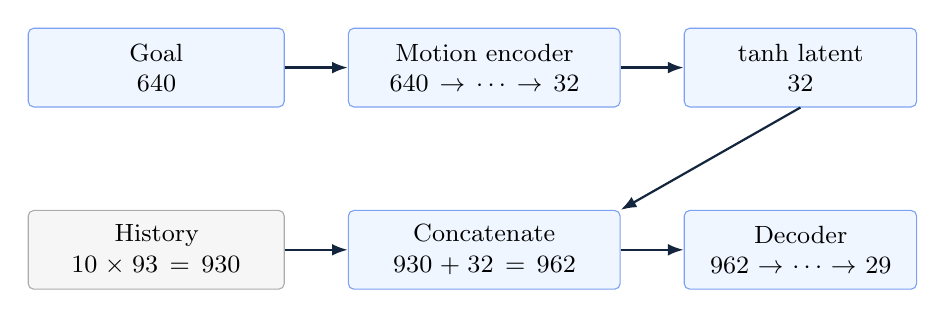
\begin{tikzpicture}[node distance=8mm and 8mm]
\node[box,text width=29mm] (goal) {Goal\\640};
\node[box,text width=31mm,right=of goal] (enc) {Motion encoder\\$640\to\cdots\to32$};
\node[box,text width=26mm,right=of enc] (latent) {$\tanh$ latent\\32};
\node[graybox,text width=29mm,below=13mm of goal] (hist) {History\\$10\times93=930$};
\node[box,text width=31mm,below=13mm of enc] (cat) {Concatenate\\$930+32=962$};
\node[box,text width=26mm,below=13mm of latent] (dec) {Decoder\\$962\to\cdots\to29$};
\draw[arr] (goal)--(enc);\draw[arr] (enc)--(latent);
\draw[arr] (hist)--(cat);\draw[arr] (latent.south)--(cat.north east);
\draw[arr] (cat)--(dec);
\end{tikzpicture}
\caption{The goal encoder and action decoder are trained end to end. The
decoder's 29 outputs are clamped to $[-10,10]$ and converted to joint-position
targets. The encoder's 32 outputs are bounded by $\tanh$.}
\end{figure}

\subsection{Normalization is part of the saved controller}
Joint angles, velocities, and orientation components have different scales. Each
normalizer tracks componentwise running means and variances using sample counts:
\begin{equation}
N(x)=\clip\left(\frac{x-\mu}{\max(\sigma,0.01)},-20,20\right).
\end{equation}
The observation, goal, world-model input, world-model output residual, and critic
input have separate statistics. The statistics are buffers, not parameters
updated by gradient descent. Their updates use no gradients, but the transformation
$N(x)$ is still differentiable with respect to $x$ away from clamp boundaries.

The world model's residual output is \emph{denormalized}; it is not subjected to
the $[-20,20]$ input clamp. Normalizers must be loaded with the weights at
evaluation time. Loading only the linear-layer matrices would change the meaning
of the controller's inputs and predictions.

The decoder and model final-layer weights start with Gaussian standard deviation
$10^{-4}$ and zero biases. Other layers use PyTorch's default initialization.
The policy is deterministic. Gaussian collection noise is added outside the
network; there is no learned action variance or log-probability head.

\subsection{Why the world model predicts 70 residuals, not 71 raw values}
The state stores four quaternion components, but an orientation change has only
three independent components. We use a rotation vector for that change. The
model predicts
\begin{equation}
\delta=[\delta p,\delta r,\delta v,\delta\omega,\delta q,\delta\dot q]
\in\R^{70},
\end{equation}
with counts $3+3+3+3+29+29$. Translational and velocity changes are expressed in
the current base frame. An analytic integration function reconstructs the next state:
\begin{align}
p'&=p+R(Q)\delta p,& Q'&=\operatorname{normalize}(Q\otimes\operatorname{Exp}(\delta r)),\\
v'&=v+R(Q)\delta v,&\omega'&=\omega+R(Q)\delta\omega,\\
q'&=q+\delta q,&\dot q'&=\dot q+\delta\dot q.
\end{align}
Predicting changes makes the output scale local to one 20~ms transition. Quaternion
integration preserves the unit-orientation representation. Position and velocity
are still predicted jointly: there is no additional exact kinematic constraint
forcing $p'=p+\Delta t\,v$ in the learned model.

\subsection{The critic's output is a scalar value}
The critic estimates discounted future reward, not immediate pose error or the
probability of falling. Its output is clamped to $[-12,12]$ as a numerical
stabilization choice. This does not mean $-12$ is a true lower bound on task
returns: penalties can make reward negative. A clamp can also limit useful
gradients when the output saturates.

The critic's inputs are still a compressed representation, not the full formal
task state $z_t$. In particular, they omit absolute root XY and any reference
information outside the preview. Two task states can therefore share a critic
input while having different true returns. The critic is an approximate value
predictor under this information restriction, not an exact Markov-state oracle.
\src{networks.py: mlp, Normalizer, WorldModel, Actor, Critic; math_utils.py: integrate}

\section{Motion data and what imitation means here}\label{sec:data}
\subsection{The data is already a robot reference}
We use the G1 CSV portion of \code{lvhaidong/LAFAN1_Retargeting_Dataset}, pinned to
revision \code{ce1572906efe6157840e8474d5a0d7aa87481e74}. This dataset is the input
to our converter, not an output of our training system. The clips have already
been retargeted to the robot. Human-to-G1 inverse kinematics and retargeting are
not being learned in this experiment.

Each original row has 36 values: root position (3), XYZW root quaternion (4), and
29 joint angles. The source sampling rate is 30~Hz. Our converter resamples at
50~Hz using linear interpolation for root/joint positions and quaternion SLERP
for orientation. It makes quaternion signs continuous and computes velocities
using finite differences and relative rotations. The resulting state is the
71-component representation introduced earlier.

The converted library contains \textbf{40 clips and 441,140 frames}, about
2.4506 hours when summed as frames divided by 50~Hz. Using $(N-1)/50$ for the
elapsed interval within each clip changes the total slightly. Source-file hashes,
joint order, quaternion convention, and the dataset revision are retained as
provenance. Clip starts and lengths prevent sampling from accidentally crossing
from one motion into the next.

\subsection{Two kinds of data with different purposes}
\begin{tabularx}{\linewidth}{@{}lXX@{}}
\toprule
Data source & Contents & Role\\
\midrule
Reference library & Desired robot states over time & Builds goals, reset poses,
and tracking-reward targets\\
Simulator replay & Robot states and \emph{executed} actions, including mistakes
and falls & Supervises the dynamics model and seeds imagined policy rollouts\\
\bottomrule
\end{tabularx}
The reference dataset does not supply the expert motor commands needed for
ordinary action-supervised behavior cloning. It tells us what motion we want,
not necessarily what PD target or torque will produce it in our particular simulator.

\subsection{Imitation through reward, rather than action labels}
A behavior-cloning objective would have the form
\begin{equation}
L_{\rm BC}=\E\big[\norm{\pi_\theta(h,g)-a^{\rm expert}}^2\big].
\end{equation}
We do not optimize this objective, and no $a^{\rm expert}$ is available to our
learner. Instead, reference states define a reward. The policy discovers commands
that lead to high reference-tracking reward under the learned dynamics, and its
actual behavior is checked in physics.

Simply setting joint targets to the reference angles is a useful baseline but
does not solve the same problem. The robot may need anticipatory balance,
compensation for limited motor effort, and recovery from existing tracking
errors. The action scale and PD target are not themselves a command for the
robot's next physical state. Kinematically plausible references are also not
automatically dynamically feasible under our robot inertias, contacts, and gains.

\subsection{Random reference-state initialization}
Training does not always begin at the first frame. It samples a clip uniformly,
then a frame uniformly before that clip's final 33 frames. The robot is initialized
to that frame's root pose, joints, and velocities, with uniform joint-position
noise of $\pm0.02$ rad. This exposes the learner to many parts of long clips
without requiring it to survive from their beginnings first.

This is not a return-weighted curriculum or an adaptive sampler. Longer clips
do not receive proportionally more clip-selection probability: the clips are
uniformly selected, then time is sampled within the chosen clip. Evaluation
starts from first frames, so its state distribution differs from collection.
\src{motions.py: prepare and MotionLibrary; environment.py: TrackingEnv.reset}

\section{Physics, the robot, and action execution}\label{sec:physics}
\subsection{The simulator is the ground truth for this experiment}
IsaacLab supplies the scene and articulation APIs. Training and all recorded
videos use \textbf{Newton with the MuJoCo Warp solver}, selected explicitly with
\code{MJWarpSolverCfg} inside \code{NewtonCfg} in the saved training source.
The Newton dependency is pinned to the public \code{newton-physics/newton}
repository at this commit:
\par\code{42f7def118c2c4299ce493457bafd4e8a22a696e}.
\par
\textbf{No DVI solver was obtained or integrated for this experiment.}
The scene is a flat floor with fixed robot and contact parameters. Policy
gradients pass through the learned neural world model, not through Newton or
MuJoCo Warp.

The shipped asset named \code{g1_29dof.usd} contains 14 extra finger joints.
Before physics import, the adapter creates a temporary flattened USD variant
that welds those finger joints at zero. Their mass stays attached. It asserts
that exactly the 29 modeled moving joints remain; the cached original asset is
not edited. Otherwise, unmodeled movable fingers would violate the intended
state/action contract.

\subsection{From normalized actions to motor targets}
For joint $j$, the network's normalized action becomes
\begin{align}
q^{\rm target}_j&=q^{\rm default}_j+\alpha_j a_j,\\
\alpha_j&=\frac{0.25\,\tau^{\rm limit}_j}{K_{p,j}},\\
K_{p,j}&=I^{\rm armature}_j(20\pi)^2,
\qquad K_{d,j}=4I^{\rm armature}_j(20\pi).
\end{align}
A useful approximation to the drive is
\begin{equation}
\tau_j\approx K_{p,j}(q^{\rm target}_j-q_j)-K_{d,j}\dot q_j,
\end{equation}
with configured effort limits. The actual implicit actuator/backend handles
execution; this approximation is not a replacement for its numerical details.

The scale does not hard-limit the actual torque to one quarter of its effort
limit. It maps a unit normalized target offset to that nominal proportional
effort contribution at the default pose. Actual position error, damping, action
magnitude, and effort saturation also matter.

Leg effort limits range from 50 to 139~Nm; shoulder/elbow/wrist-roll joints use
25~Nm, and wrist pitch/yaw use 5~Nm. The default pose bends the hips, knees,
ankles, shoulders, and elbows. Exact armatures, gains, and name mappings live in
\code{robot_cfg()} rather than being inferred from the policy output.

\subsection{Training noise and deterministic evaluation}
The actor output is deterministic, but collection executes
\begin{equation}
a_t^{\rm exec}=\clip(\pi_\theta(h_t,g_t)+\epsilon_t,-10,10),
\qquad\epsilon_t\sim\mathcal N(0,0.1^2I).
\end{equation}
Replay stores this executed action. The smoothness penalty and the following
observation's previous-action field also use it. Training sensor noise affects
observations; it does not alter the logged physical state used to supervise
the model. Imagined rollouts use deterministic actor actions and noisy
observations, without adding the Gaussian action perturbation.

Evaluation and the recorded videos disable observation, action, and reset noise.
This separates tracking quality under a fixed protocol from exploration behavior.

\begin{center}
\begin{tabularx}{\linewidth}{@{}lX@{}}
\toprule
Physics setting & Configured value\\
\midrule
Parallel training worlds & 256, spaced 4 meters apart\\
Physics / control rate & 200 / 50~Hz; four physical steps per control action\\
Integrator & \code{implicitfast}\\
Solver / line-search cap & 10 / 50 iterations\\
Configured contact capacities & \code{nconmax=150}, \code{njmax=500}\\
Contact generation & Newton contacts; \code{use_mujoco_contacts=False}\\
Contact margin, stiffness, damping & $0$, $160{,}000$, $1{,}100$\\
Friction / restitution & 1.0 / 0.0 for robot and floor\\
Self-collision & Enabled physically\\
Physical-parameter randomization & None in this run\\
\bottomrule
\end{tabularx}
\end{center}
\src{environment.py: robot_cfg, simulation_cfg, TrackingEnv.step}

\section{Rewards, kinematics, and failure}\label{sec:rewards}
\subsection{Why joint angles alone are not the whole reward}
A floating robot can have nearly the correct internal joint angles while its
base is displaced or incorrectly oriented. We therefore compare poses and
velocities of 14 tracked body links, plus the root pose. These bodies include
the pelvis, torso, and bilateral hip-roll, knee, ankle-roll, shoulder-roll,
elbow, and wrist-yaw links.

Forward kinematics maps a root state and joint configuration to body positions
and orientations. With velocities, it also computes body linear/angular
velocities. Our PyTorch kinematic tree is extracted from the finalized Newton
model, including parent/child joint-frame offsets. The calculations are
differentiable, so imagined body-tracking rewards can send gradients back to
predicted joints and base motion.

The same kinematics processes robot and reference states. Reference kinematics
can be precomputed outside the policy's gradient path. Kinematic differentiation
is not differentiating the contact solver: it describes how a pose determines
body geometry, not how forces cause that pose to evolve.

\subsection{The reward equation}
For a mean squared body-position error, define
\begin{equation}
e_p^2=\frac{1}{14}\sum_b\norm{p_b-\bar p_b}^2,
\qquad R_p=\exp(-e_p^2/0.3^2).
\end{equation}
The analogous orientation error uses the rotation logarithm; linear and angular
velocity errors use the corresponding body velocities. The positive terms are
\begin{equation}
T=R_p+R_R+R_v+R_\omega+0.5R_{p,\rm root}+0.5R_{R,\rm root},
\end{equation}
with characteristic scales $0.3$~m for position, $0.4$~rad for orientation,
$1.0$~m/s for linear velocity, and $3.14$~rad/s for angular velocity. The
implementation exponentiates the body-mean squared error, rather than averaging
an exponential computed separately at each body.

Let $q_j^{\rm low},q_j^{\rm high}$ be soft joint limits. The complete step reward is
\begin{align}\label{eq:reward}
r_{t+1}=0.02\Big[&T(s_{t+1},\bar s_{c,k_t+1})
-0.1\sum_j(a_{t,j}-a_{t-1,j})^2\\
&-2\sum_j\big(\max(q_{t+1,j}-q_j^{\rm high},0)
+\max(q_j^{\rm low}-q_{t+1,j},0)\big)\Big].\nonumber
\end{align}
The factor $0.02$ is the control interval. Positive term weights sum to 5, giving
a maximum reward of $0.1$ per step when tracking is perfect and penalties vanish.
Rewards can be negative. This maximum explains the evaluation normalizer; it
does not imply that all normalized returns must mathematically lie above zero.

\begin{idea}{How to read an exponential tracking term}
If one error equals its characteristic scale and the others are zero, that term
is $e^{-1}\approx0.368$. Near perfect tracking, its score approaches one. The
gradient changes continuously with the error, making it useful for training
through predicted states. The scales determine how forgiving each term is.
\end{idea}

Body/root positions are compared in world-aligned coordinates after removing
each world's placement offset. There is no fresh XY/yaw realignment of the
reference at every step. There is also no explicit self-collision reward penalty,
even though physical self-collision is enabled.

\subsection{Hard failures are reference relative}
Define
\begin{align}
h&=|p_z-\bar p_z|,\\
e&=|[R(Q)^T(0,0,-1)]_z-[R(\bar Q)^T(0,0,-1)]_z|.
\end{align}
The simulator declares failure when $h>0.25$~m or $e>0.8$. The second expression
is a difference of gravity-vector $z$ components, not a direct angle threshold
in radians. A reference that is intentionally lying down is not automatically
a failed reference. There is no separate end-effector-distance failure criterion.

\subsection{Soft termination makes survival trainable}
A hard indicator has no useful derivative away from its threshold. Imagination
uses a smooth approximation instead:
\begin{align}
d_h&=\sigma(100(h-0.25)),&d_e&=\sigma(30(e-0.8)),\\
d&=1-(1-d_h)(1-d_e).
\end{align}
The quantity $d$ behaves as a soft termination probability in the objective.
It is an analytic surrogate, not the calibrated output of a learned fall
classifier. Multiplying future return by $1-d$ lets the actor receive gradients
for approaching failure boundaries, rather than only a discrete penalty after
crossing them. At $h=0.25$ and a negligible tilt contribution, $d$ is about 0.5.
\src{task.py: Kinematics, TrackingTask.reward, TrackingTask.termination}

\section{The training loop and its replay buffer}\label{sec:loop}
\subsection{Three updates, three different learning signals}
It helps to explicitly separate the supervised dynamics problem from the
reinforcement-learning control problem:
\begin{center}
\begin{tabularx}{\linewidth}{@{}lXXX@{}}
\toprule
Update & Data / target & Parameters changed & Held fixed\\
\midrule
World-model fit & Real transition sequences & Dynamics $\phi$ & Logged actions and states\\
Actor improvement & Imagined tracking return & Encoder + decoder $\theta$ & Dynamics/critic weights, reference data\\
Critic fit & Detached imagined lambda returns & Value network $\psi$ & Target returns, imagined input samples\\
\bottomrule
\end{tabularx}
\end{center}
The model is updated throughout learning. It is frozen only inside an actor
update. There is no initial world-model pretraining followed by permanent
freezing for the rest of the experiment.

\subsection{Collecting real evidence}
For one outer-loop iteration, each of 256 worlds takes one 20~ms control step.
The collector builds goals, updates actor input statistics, selects and perturbs
actions, steps physics, and records
\begin{equation}
(s_t,s_{t+1}^{\rm pre-reset},a_t,a_{t-1},\text{episode ID},c,k_t).
\end{equation}
Only after capturing that transition does it reset failed or timed-out worlds.
This ordering is essential. If a fall's successor were replaced with a reset
pose, the world model would be taught that a bad action magically restores the
robot, corrupting both prediction and policy gradients.

The replay buffer is a GPU ring with 256 time slots per world, holding
$256\times256=65{,}536$ transitions, about 51.5 MiB. It retains up to 5.12 seconds
of recent transitions per world; it is not a permanent archive of all training
experience.

Eight-step model windows must lie within one episode. A terminal transition can
be the last element, retaining the actual fallen state. Imagined starts sample
replay states and reconstruct episode-local observation histories. Missing
history near an episode or buffer boundary is padded with the earliest valid
observation. The reconstruction applies fresh observation noise.

\subsection{What one scheduled update event does}
An update-credit counter increases by 0.4 after each collection iteration.
Whenever it reaches one, the loop runs the following and subtracts one:
\begin{enumerate}
\item Ten dynamics optimizer steps, each using 256 eight-step windows.
\item One actor optimizer step, using 512 imagined rollouts of length 32.
\item Twenty critic optimizer steps: five epochs, with four shuffled minibatches per epoch.
\end{enumerate}
Thus there are about two update events for every five simulator iterations.
The setting \code{utd=0.4} describes this scheduler, not a literal ratio of
imagined transitions to real transitions or a ratio of all optimizer steps to
new samples.

\begin{idea}{A concrete amount of work}
Five collection iterations produce $5\times256=1{,}280$ real transitions.
Two update events produce $2\times512\times32=32{,}768$ imagined policy transitions,
20 dynamics optimizer steps, two actor steps, and 40 critic steps. Replay samples
can be reused. These different counts should not all be called ``training steps.''
\end{idea}
\src{learner.py: collect, fit_model, improve_policy; replay.py; train.py: training loop}

\section{Learning the world model}\label{sec:modeltraining}
\subsection{The supervised target is what physics actually did}
For an initial logged state and eight executed actions, the model rolls itself
forward autoregressively:
\begin{equation}
\hat s_0=s_0,\qquad\hat s_{j+1}=F_\phi(\hat s_j,a_j),
\quad j=0,\ldots,7.
\end{equation}
At later steps the input is the previous \emph{prediction}, not the logged
ground-truth state. This exposes accumulated prediction error during training,
which is closer to how the model will be used in imagination.

Define $\Delta(s,s')$ as the 70-component local state difference used by the
residual representation: base-frame translation/velocity differences, a
relative rotation vector, and joint differences. The loss is
\begin{equation}\label{eq:modelloss}
L_{\rm model}=\frac{1}{8B\cdot70}
\sum_{b=1}^B\sum_{j=0}^7
\norm{\frac{\Delta(s_{b,j+1},\hat s_{b,j+1})}{\sigma_\delta}}^2,
\qquad B=256.
\end{equation}
The division is componentwise by running residual standard deviations. This
prevents numerically large units from dominating the objective simply by scale.
Input/output normalizer statistics are updated from the first logged transition
of each sampled window before the optimizer step.

\subsection{What the model learns implicitly}
The model predicts a \emph{controlled} transition. Because actions are converted
to PD targets before physics, the model must capture the net effects of that
drive, robot inertias, gravity, and contacts over 20~ms. It does not explicitly
output forces, contact points, or a contact-mode label.

Reference goals are absent from Equation~\eqref{eq:modelloss}. A simulator state
can be off the reference trajectory, and those off-target states are useful
training examples. The model needs to predict what happens when the policy
makes mistakes, not only memorize ideal motion trajectories.

\subsection{Why prediction accuracy is not the whole story}
One-step errors can accumulate over a 32-step policy rollout. More subtly, the
actor uses derivatives of the learned function. Low average prediction error
does not guarantee accurate action derivatives, especially around contact
transitions or outside the replay distribution. A policy can exploit model
errors by finding states that look rewarding in imagination but fail in physics.

Short rollouts, continued real-data collection, repeated model fitting, and
actual simulator evaluation help manage this problem. They do not eliminate
model bias. Our model is deterministic and has no ensemble-based uncertainty
estimate in this experiment.
\src{learner.py: model_loss, fit_model, prediction_errors; math_utils.py: state_delta}

\section{Training the actor by differentiating imagined futures}\label{sec:bptt}
\subsection{The imagined loop is closed loop too}
For each of 512 replay starts, reconstruct its ten-frame observation history.
Then repeat for $H=32$ steps:
\begin{align}
g_j&=G(\hat s_j,c,k+j),\\
a_j&=\pi_\theta(\hat h_j,g_j),\\
\hat s_{j+1}&=F_\phi(\hat s_j,a_j),\\
\hat r_{j+1}&=r(\hat s_{j+1},\bar s_{c,k+j+1},a_j,a_{j-1}).
\end{align}
Append an observation of $\hat s_{j+1}$ to the imagined history and recompute the
next goal. These actions are not a fixed sequence computed once at the beginning;
the actor responds to each predicted state.

\begin{figure}[htbp]
\centering
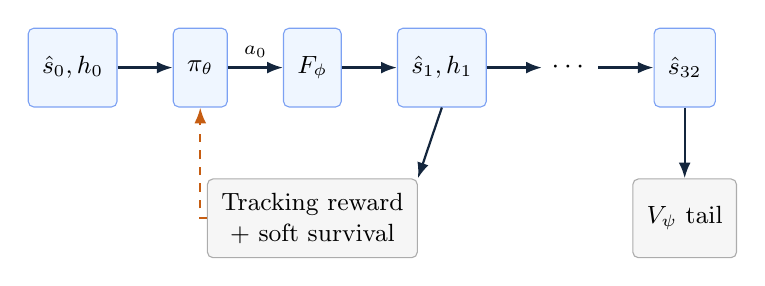
\begin{tikzpicture}[node distance=9mm and 7mm]
\node[box] (s0) {$\hat s_0,h_0$};
\node[box,right=of s0] (p0) {$\pi_\theta$};
\node[box,right=of p0] (f0) {$F_\phi$};
\node[box,right=of f0] (s1) {$\hat s_1,h_1$};
\node[draw=none,right=of s1] (dots) {$\cdots$};
\node[box,right=of dots] (sh) {$\hat s_{32}$};
\node[graybox,below=of f0] (r) {Tracking reward\\+ soft survival};
\node[graybox,below=of sh] (v) {$V_\psi$ tail};
\draw[arr] (s0)--(p0);\draw[arr] (p0)--node[above,font=\scriptsize]{$a_0$}(f0);
\draw[arr] (f0)--(s1);\draw[arr] (s1)--(dots);\draw[arr] (dots)--(sh);
\draw[arr] (s1.south)--(r.north east);\draw[arr] (sh)--(v);
\draw[grad] (r.west) -| (p0.south);
\end{tikzpicture}
\caption{An abbreviated unroll. The same actor and world-model weights are reused
at every step. Future reference inputs are supplied at every actor evaluation.
Only actor weights change in this backward pass; gradients pass through model
operations and the terminal critic.}
\end{figure}

\subsection{The survival-weighted return}
Let $m_j$ be one while the reference transition is still inside its clip and
zero afterwards. Define
\begin{equation}
c_0=1,\qquad c_{j+1}=c_j(1-d_{j+1})m_j,
\end{equation}
where $d_{j+1}$ is soft termination at the predicted successor. The objective is
\begin{equation}\label{eq:actorobjective}
J=\sum_{j=0}^{H-1}\gamma^j c_j m_j\hat r_{j+1}
+\gamma^H c_H V_\psi(\hat s_H,g_H),\qquad\gamma=0.99.
\end{equation}
The terminal critic notation here abbreviates its actual concatenated
709-component input. The current step's reward is weighted by survival
\emph{before} that transition; its soft failure reduces later contributions.
The clip-end mask prevents fictitious returns past the reference's end.

The actor minimizes
\begin{equation}
L_{\rm actor}=-\frac{\operatorname{mean}_{\rm batch}J}
{\sum_{j=0}^{31}\gamma^j}.
\end{equation}
The denominator is approximately 27.5. It rescales gradients without changing
which policy maximizes this objective for a fixed horizon and discount.

\subsection{How the gradient reaches an earlier action}
Consider a simplified memory-free policy $A_\theta(s)$ at a fixed reference
schedule. Its total dependence on state includes any state-dependent goal
construction. Applying the chain rule gives
\begin{equation}\label{eq:chain}
\frac{d\hat s_{j+1}}{d\theta}
=\left(F_s+F_a A_s\right)\frac{d\hat s_j}{d\theta}
+F_a A_\theta.
\end{equation}
$F_s$ and $F_a$ are model derivatives with respect to state and action.
$A_\theta$ is the policy derivative with respect to its weights. In the real
implementation, one can extend the state in this equation to include the history
buffer and previous action; automatic differentiation handles those paths too.

An early action changes the next state, which changes the next observation,
goal features, action, reward, survival, and ultimately the critic's tail value.
Backpropagation through time accumulates all those consequences into an actor
gradient. There are no policy-likelihood ratios or PPO advantage ratios in this
update.

\subsection{Comparison with the familiar model-free loop}
In a typical PPO setup, the actor is updated from sampled simulator trajectories,
estimated advantages, and derivatives of action log probabilities. The simulator
is treated as a black box. Our code instead constructs a differentiable predicted
trajectory and uses derivatives of predicted rewards with respect to actions
and policy weights.

\begin{tabularx}{\linewidth}{@{}lXX@{}}
\toprule
Aspect & Typical model-free PPO & This implementation\\
\midrule
Actor training signal & Likelihood-ratio surrogate with estimated advantages &
Backpropagated imagined reward and tail value\\
Learned transition model & Not required & Required and updated online\\
Simulator derivatives & Not required & Not required\\
Critic targets & Usually based on real sampled trajectory rewards &
Detached model-imagined lambda returns\\
Runtime controller & A policy forward pass & Encoder + decoder forward pass\\
\bottomrule
\end{tabularx}
Both approaches can be goal conditioned and can use dense imitation rewards.
The defining change here is the actor's gradient estimator and its dependence
on a learned transition function. Our experiment does not include a controlled
PPO baseline establishing a measured speedup.

\subsection{A two-step worked example}
To isolate delayed credit assignment, consider a one-dimensional toy mass. This
is an explanatory example, not the G1's actuator equation. With forward Euler,
\begin{align}
p_{j+1}&=p_j+\Delta t\,v_j,\\
v_{j+1}&=v_j+\Delta t\,a_j/m.
\end{align}
An action $a_0$ has no effect on $p_1$ under this discretization, but it affects
$v_1$ and therefore $p_2$:
\begin{equation}
\frac{\partial p_1}{\partial a_0}=0,\qquad
\frac{\partial p_2}{\partial a_0}=\frac{\Delta t^2}{m}.
\end{equation}
For a two-step target reward $r_2=-(p_2-p^*)^2$,
\begin{equation}
\frac{\partial r_2}{\partial a_0}
=-2(p_2-p^*)\frac{\Delta t^2}{m}.
\end{equation}
If $p_2<p^*$, the derivative is positive: increasing the first action improves
the later target error. For $p_2=0$, $p^*=0.1$, $m=1$, and $\Delta t=0.02$,
the derivative is $8\times10^{-5}$. The calculation connects a later reward to
an earlier action even though the first position change had no action gradient.
The humanoid version applies the same chain-rule idea through a learned
high-dimensional transition function and a much richer reward.

\subsection{Frozen weights do not mean disabled derivatives}
During the actor update, the code freezes model and critic \emph{parameters}.
It does not enclose their forward operations in a blanket \code{no_grad()}.
The derivatives $F_a$, $F_s$, and the critic's input derivative are still needed.
Otherwise, the actor would lose the path connecting its commands to future reward.

Similarly, reference arrays and sampled replay states are constants for an
update, but predicted states are not detached at each step. The critic-fitting
targets are deliberately detached later; that is a different update with a
different purpose.

\begin{caution}{These are surrogate gradients}
``Analytic policy gradients'' here means gradients obtained by automatic
differentiation through the neural surrogate and analytic task calculations.
They are not exact derivatives of Newton/MJWarp contact dynamics. No backward
pass goes through a real simulator transition in this implementation.
\end{caution}

\subsection{Why this is not runtime model predictive control}
The imagined rollout is a training graph. Its optimizer changes shared policy
weights, amortizing useful control behavior across future executions. At runtime
there is no per-step optimization over a fresh action sequence. The controller
uses a single actor forward pass and then observes what the robot actually did.
\src{learner.py: frozen, _imagined_step, improve_policy; networks.py: goal}

\section{The critic and lambda-return targets}\label{sec:critic}
\subsection{Why a 0.64-second rollout needs a tail estimate}
Good balance decisions can have consequences beyond the 32 imagined steps.
Without a tail estimate, the policy has less incentive to preserve a state that
is valuable just after the rollout ends. The critic approximates the remaining
discounted return, letting a short rollout represent a longer-term objective.

The critic is goal conditioned because the future task matters. Its state
features alone cannot distinguish ``prepare to stop'' from ``prepare to run''
when the robot is currently in the same pose.

At our discount, $\gamma^{32}\approx0.725$, so the tail has substantial weight
even before accounting for survival. The geometric discount sum is
$1/(1-\gamma)=100$ control steps, suggesting a discount timescale of about
two seconds. A hypothetical indefinitely perfect controller with reward 0.1
per step would have discounted value $0.1/(1-0.99)=10$.

\subsection{The targets used by this code}
For detached imagined rewards, continuation factors $b_j=(1-d_{j+1})m_j$, and
critic values $V_j$, initialize $Y_H=V_H$ and recurse backward:
\begin{equation}\label{eq:lambda}
Y_j=\hat r_{j+1}m_j+\gamma b_j\left[(1-\lambda)V_{j+1}+\lambda Y_{j+1}\right],
\qquad\lambda=0.95.
\end{equation}
For $\lambda=0$, this is a one-step bootstrapped target. For $\lambda=1$, it
uses the imagined rewards all the way to the horizon and then the terminal
bootstrap. Intermediate values mix those horizons. The configuration field is
named \code{gae_lambda}, but this code uses it to construct value-regression
lambda returns, not PPO policy-advantage ratios.

The critic loss is
\begin{equation}
L_{\rm critic}=\operatorname{mean}\big(V_\psi(\text{input}_j)-\sg(Y_j)\big)^2.
\end{equation}
The target is fixed across five epochs. There are $512\times32=16{,}384$
imagined state/value examples, shuffled into four minibatches per epoch, giving
20 critic optimizer steps for one actor update. There is no separate target
critic or exponential-moving-average copy.

\subsection{Why the gradient treatment differs from the actor's}
For actor improvement, a differentiable terminal value tells the actor how
changing its resulting state could improve future return. For critic fitting,
the target is held constant so the network learns to predict that target rather
than move the target through the same backward pass. These two uses of the
critic are compatible because they happen in separate optimization stages.

The critic is trained on model-generated trajectories. It therefore shares
exposure to model bias. A small critic loss only means it fits those targets;
it does not independently prove that real long-horizon behavior is correct.
\src{learner.py: improve_policy; networks.py: Critic}

\section{Putting the learning procedure into practice}\label{sec:practical}
\subsection{Pseudocode with the three learning signals separated}
The following is conceptual pseudocode. It summarizes the control flow; it is
not intended to be pasted into Python as the exact public API.
\begin{tcolorbox}[colback=gray!4,colframe=gray!50,title=One online learning loop]
\small
\begin{enumerate}
\item Load the motion library and the validated starting checkpoint. Start fresh
physics worlds and refill replay.
\item For every outer simulator iteration:
\begin{enumerate}
\item Build goals from each world's clip/frame and current orientation.
\item Evaluate the actor, add collection action noise, and step the simulator.
\item Store the actual transition, including its pre-reset successor.
\item Reset only worlds that failed or timed out.
\item Add 0.4 to update credit. If credit is at least one:
\begin{enumerate}
\item Subtract one; fit the model on ten batches of real eight-step sequences.
\item Sample 512 replay starts and reconstruct observation histories.
\item Freeze model/critic weights, unroll 32 steps, and update the actor from
the negative survival-weighted return.
\item Detach imagined samples; form lambda returns and fit the critic for
five epochs of four minibatches.
\end{enumerate}
\item Periodically evaluate in real physics and save the learner state.
\end{enumerate}
\end{enumerate}
\end{tcolorbox}

\subsection{Optimizer settings and gradient clipping}
\begin{center}
\small
\begin{tabularx}{\linewidth}{@{}lXXX@{}}
\toprule
Setting & World model & Actor & Critic\\
\midrule
Optimizer & Adam & Adam & Adam\\
Initial learning rate & $2\times10^{-4}$ & $2\times10^{-4}$ & $2\times10^{-4}$\\
Adam betas & $(0.9,0.999)$ & $(0.9,0.95)$ & $(0.9,0.999)$\\
Global gradient-norm cap & 1.0 & 1.0 & 1.0\\
Additional componentwise cap & None & $\pm0.1$ after norm cap & None\\
Steps per update event & 10 & 1 & 20\\
\bottomrule
\end{tabularx}
\end{center}
The shared learning-rate schedule, indexed by simulator iteration $i$, is
\begin{equation}
\eta(i)=2\times10^{-4}\left[0.03+0.97\frac{1+\cos(\pi\min(i/250000,1))}{2}\right].
\end{equation}
After iteration 250,000 it remains at $6\times10^{-6}$. This schedule is not
indexed by the much larger number of model or critic optimizer steps.

Losses and gradients are checked for finite values. Logged gradient norms are
measured \emph{before} clipping, so a logged value above one does not mean the
gradient cap failed. Componentwise action and normalization clamps can also
saturate; the network is differentiable almost everywhere rather than everywhere.

\subsection{The scale of the completed experiment}
The main loop executed 320,000 iterations, or
$320{,}000\times256=81{,}920{,}000$ real transitions. This is about 455 aggregate
simulated robot-hours at 50~Hz, spread across worlds and many short episodes.
It is different from the 2.45 hours of reference motion being reused.

Approximately 128,000 main-loop actor updates imply about 2.10 billion imagined
policy transitions. Dynamics fitting additionally processes about 2.62 billion
predicted training-window transitions, with repeated replay sampling. These
are computational-work counts, not distinct independent observations of physics.
The final saved update counter is 128,200, including the 200 readiness updates.

The run used full-width networks on an NVIDIA RTX PRO 4500 Blackwell Server
Edition with 32~GB of GPU memory. It used Python 3.12, PyTorch
\code{2.11.0+cu130}, Warp 1.17, and the repository's pinned Newton/MuJoCo Warp
dependencies. PyTorch compilation wraps the model-window loss and an imagined
step. The code uses float32 with high float32-matmul precision; there is no
explicit autocast/gradient-scaler training path. Peak logged PyTorch allocation
was about 2.34~GiB; this excludes allocations owned by other GPU libraries and
processes.
The experiment's random seed was 42.

\subsection{What a checkpoint preserves}
Saved checkpoints include the three networks, running normalizers, all three
optimizers, counters, random-generator states, selected motion names, and data
provenance. They do not include replay, physical robot state, or solver warm-start
buffers. Resume creates fresh episodes and refills replay, so it continues
learning without replaying the exact previous physical trajectory bit for bit.

During the run, \code{last.pt} was atomically overwritten every 500 iterations.
There is no automatic best-checkpoint archive. A high historical evaluation does
not imply those exact weights remain available. The video batches separately
retained their immutable recording checkpoints.
\src{learner.py: optimizer_step, save, load; train.py: train and learning-rate schedule}

\section{Validation and results from our completed run}\label{sec:results}
\subsection{Why there was a readiness stage}
A plausible training loss is insufficient if the state coordinates, joint
ordering, reset logic, or reward kinematics are wrong. Before the full launch,
readiness checked the physical state contract, exactly 29 modeled joints,
kinematics against simulator body data, and preservation of terminal successors.
It also verified finite nonzero policy gradients, a repeated evaluation,
checkpoint reload plus an optimizer update, and memory headroom.

Maximum observed discrepancies between the differentiable kinematics and
simulator body data were about $4.86\times10^{-6}$~m for position,
$2.70\times10^{-7}$~rad for orientation, $5.04\times10^{-6}$~m/s for linear
velocity, and $4.05\times10^{-6}$~rad/s for angular velocity. These checks target
coordinate and tree-consistency errors; they do not prove the learned contact
model's action derivatives are correct.

\begin{center}
\begin{tabularx}{\linewidth}{@{}Xrr@{}}
\toprule
Readiness measurement & Before & After\\
\midrule
Held-out eight-step root-position component RMSE (m) & 0.05553 & 0.01435\\
Held-out eight-step joint-position component RMSE (rad) & 0.20082 & 0.04703\\
Mean five-second simulator return & 0.07599 & 0.44876\\
Failed five-second motion windows & 40/40 & 15/40\\
\bottomrule
\end{tabularx}
\end{center}
The hold-out refers to a separate block of collected transitions, not unseen
reference motion clips. The full experiment loaded this validated learner,
including its trained weights and optimizer states. Its iteration-zero evaluation
is therefore already warm-started, approximately 0.4485, not an untrained baseline.

\subsection{The exact periodic evaluation protocol}
Every 2,000 main-loop iterations, each selected clip starts at its first frame
with noise disabled. The controller is followed for 250 transitions, or five
seconds. Failure stops that trajectory from contributing later reward. The score
is the undiscounted reward sum divided by
\begin{equation}
0.1\min(250,\text{clip length}-1).
\end{equation}
The 256 worlds contain six or seven replicas of each of the 40 clips. Scores
are averaged within clip, then equally across clips. A clip is marked failed
if any replica fails. These replicas are not a deliberately randomized robustness
test.

\begin{caution}{What ``0/40 failures'' actually says}
For the final training result it means zero failed \emph{five-second first-frame
windows on these 40 training clips}. It does not mean every complete motion was
successfully tracked, or that unseen motions, perturbed dynamics, and hardware
were validated. A separate full-clip evaluation mode exists but is not the
protocol represented by the final reported score.
\end{caution}

\subsection{Final result and the training trajectory}
The run finished at 320,000 iterations after approximately 21 hours 26 minutes.
The final recorded evaluation is \textbf{0.93487 normalized return with 0/40 failed
windows}. The immediately preceding evaluation of the same final iteration was
0.93489, also with zero failures. Small numerical differences can accumulate
during repeated physics execution.

The best logged periodic score was \textbf{0.96501 at iteration 290,000}. Thus
the final checkpoint is not the highest-scoring one in the log. At iteration
300,000, the score temporarily fell to 0.62367 with 16 failed windows; it recovered
to 0.95670 with no failures at 302,000. These fluctuations are visible in the
raw evaluation curve and should not be hidden by a smoothed training loss.

\begin{figure}[htbp]
\centering
\includegraphics[width=\linewidth]{figures/training_results.pdf}
\caption{The completed run's actual simulator evaluations. The horizontal axis
starts at the first full-run evaluation, after readiness. This includes a fixed
long training budget and periodic evaluations; it is not a matched time-to-target
benchmark against the paper.}
\end{figure}

\begin{figure}[p]
\centering
\includegraphics[width=0.97\linewidth,height=0.84\textheight,keepaspectratio]{figures/final_motion_returns.pdf}
\caption{Final five-second return for each motion. All 40 windows passed the hard
failure checks, but scores still vary. The weakest final window is
\code{sprint1_subject4}, approximately 0.659. Passing a failure threshold is not
the same as accurate tracking.}
\end{figure}

\subsection{How the 40-video batch differs from final evaluation}
All 40 videos use the separately saved \textbf{299,000} checkpoint, rather than
the final 320,000 checkpoint. Each contains 1,000 frames at 50 fps: 20 seconds
of playback. The first frame shows the initial state, so there are 999 executed
control transitions, spanning 19.98 seconds of physical evolution.

These are single-world, policy-controlled Newton/MJWarp rollouts, with no action,
observation, or reset noise and no resets after failures. Their normalized score
divides the 999 step rewards by $999\times0.1$. All 40 videos decoded correctly,
and none crossed a hard tracking-failure threshold. The mean score is 0.88645,
with range 0.62501--0.97469.

Those values should not be directly compared with the final 0.93487 as if only
the policy changed: the checkpoint, horizon, and rollout protocol differ. The
20-second recordings cover longer prefixes, but they still do not cover the full
2.45-hour library. They contain about 13 minutes 20 seconds of playback in total.

\subsection{Interpreting the other monitoring curves}
\begin{tabularx}{\linewidth}{@{}lX@{}}
\toprule
Metric & What a change means, and what it does not establish\\
\midrule
Model loss & Eight-step normalized replay training error; not a held-out test
of long-horizon dynamics or derivatives\\
Actor loss & Negative imagined return with survival and a critic tail; not the
actual simulator evaluation score\\
Critic loss & Error fitting detached imagined targets; not independent real
long-horizon validation\\
Simulator reward & Instantaneous mean noisy-collection reward across worlds\\
Imagined reward & Mean imagined reward from replay starts; samples a different
distribution than collection\\
Failure fraction & Fraction of worlds failing on that control step; not an
episode-level failure probability\\
Imagined survival & Mean product of soft continuation weights; not measured
physical survival probability\\
\bottomrule
\end{tabularx}
In particular, subtracting mean simulator and imagined rewards does not isolate
model error, because their state/action samples differ.

\subsection{Why the paper's ``three hours'' is not our stopping time}
The project reports a three-hour time to surpass its baseline on one H100,
using a much larger motion benchmark and full-motion evaluation; its checkpoint
evaluation time is excluded~\cite{project}. Our experiment ran a fixed 320,000
iteration budget on a different GPU, with smaller batches and a five-second
evaluation protocol. The paper's time-to-target statement is therefore not a
promise that our chosen budget should finish in three hours. Conversely, our
early short-window scores cannot establish a matched reproduction of that
benchmark. Throughput and early stopping would need a separate controlled study.
\src{runs/lafan1_full/metrics.jsonl; runs/readiness/readiness.json; videos/all_clips/metadata.json and validation.json}

\section{What transfers, what is missing, and what to test next}\label{sec:limits}
\subsection{The current scope}
This experiment establishes a working path for learning a reference-conditioned
G1 controller using an online learned dynamics model, analytic tracking rewards,
and BPTT policy gradients. It does not establish exact replication of the
authors' unpublished implementation or benchmark-scale compute results.

Explicitly absent from this run are BONES-SEED-scale data, physical-parameter
domain randomization, adaptive return-based reset sampling, downstream
velocity-command skill learning, a matched PPO comparison, and hardware transfer.
The physics backend is Newton/MJWarp. Robot inertias, geometry,
residual encoding, goal features, normalization, value clamping, and batch sizes
are part of our particular implementation choices.

\subsection{Generalization is an evaluation question}
One shared policy can condition on many references, but that architecture alone
does not prove it can follow an unseen motion. A useful next experiment would
reserve whole motion clips or subjects, keep them out of policy training, and
evaluate them under a stated protocol. A dynamics hold-out made from different
transitions of the same training motions answers a different question.

Similarly, observation/action noise during training is not physical-parameter
randomization. To evaluate robustness to mass, friction, delays, pushes, or model
error, those quantities need explicit perturbation experiments and matched
metrics. Our state-only model has no randomized-physics context input.

\subsection{A sensible evidence ladder}
\begin{enumerate}
\item Verify physical coordinates, joints, units, resets, and terminal replay.
\item Verify held-out prediction and finite action-to-return gradients.
\item Verify real-physics tracking improvement, rather than only imagined return.
\item Evaluate complete motion clips, keeping best-checkpoint selection explicit.
\item Test held-out motions and deliberately perturbed physical conditions.
\item Address orientation estimation, control timing, safety limits, and system
identification before any hardware claim.
\end{enumerate}
We have evidence for the early stages and prefix tracking across the training
library. The later stages remain separate work.

\section{Check your understanding}\label{sec:questions}
Try answering the following without looking back, then compare with the explanations.
\begin{enumerate}
\item \textbf{Two different desired motions, identical sensor history.}
The actions can differ because $g$ differs in $\pi_\theta(h,g)$. No weights need
to change for that difference to occur.
\item \textbf{The same physical state and action, but a different motion label.}
The fixed-physics world model should predict the same next physical state. The
reward and value can differ because the task reference differs.
\item \textbf{A frozen dynamics model during a policy update.}
Its weights are constants for that backward pass, but its state/action
derivatives are still used. Disabling all derivatives through its forward
operation would break the actor's dynamics gradient path.
\item \textbf{Forty clips and one 32-dimensional latent.}
The latent is not a 40-way class label. It is a continuous feature vector
computed from a moving reference preview by a shared learned encoder.
\item \textbf{Reference joint positions versus expert actions.}
Reference positions say where joints should be; they do not specify the motor
commands needed to reach them under contact dynamics. Our actor is trained from
tracking return, not a joint-angle-as-action cloning target.
\item \textbf{Perfect imagined tracking with poor simulator tracking.}
This can indicate model bias or policy exploitation of the model. Model
training loss and critic loss alone cannot rule it out.
\item \textbf{Zero final failed windows.}
That is a statement about the measured five-second protocol. It does not imply
zero failures over every full clip or under disturbances.
\item \textbf{Why the critic sees the goal.}
The value of a state depends on the desired future. A balanced standing pose
has different consequences when the upcoming motion is a pause versus a sprint.
\end{enumerate}

\appendix
\section{Notation and glossary}\label{app:notation}
\begin{longtable}{@{}p{0.20\linewidth}p{0.75\linewidth}@{}}
\toprule Symbol / term & Meaning\\\midrule\endhead
$x_t$ & Full simulator physical state, including internal numerical state when relevant.\\
$s_t$ & Extracted 71-number robot pose/velocity state.\\
$\bar s_{c,k}$ & Desired reference state of clip $c$ at frame $k$.\\
$\hat s_t$ & State predicted in a neural-model rollout.\\
$q,\dot q$ & 29 internal joint angles and angular velocities.\\
$Q,R(Q)$ & Root XYZW quaternion and its rotation matrix.\\
$o_t,h_t$ & One 93-number observation and ten-observation history.\\
$g_t$ & 640-number reference preview, including state-relative orientations.\\
$u_t$ & Learned 32-number encoded goal.\\
$a_t$ & Normalized 29-number joint-setpoint command.\\
$\theta,\phi,\psi$ & Actor, world-model, and critic parameters.\\
$\gamma$ & Per-control-step discount factor, 0.99.\\
$\lambda$ & Lambda-return mixing factor, 0.95.\\
$d,c_j,m_j$ & Soft termination, accumulated survival, and clip-end mask.\\
Goal conditioning & Supplying desired-task information as an input to a shared function.\\
World model & A learned function predicting physical state transitions.\\
Imagination & Rolling the controller through a learned transition model.\\
BPTT & Applying the chain rule through multiple successive uses of shared networks.\\
Bootstrap & Replacing an unobserved return tail with a learned value estimate.\\
Detached target & A numerical learning target through which this update sends no gradient.\\
Autoregressive & Feeding a model's previous prediction into its next prediction.\\
Closed loop & Choosing the next action from the latest actual or predicted observation.\\
Retargeting & Converting source motion to the target robot's joints and geometry.\\
PD target & A desired joint position acted on by a feedback drive, not a physical teleport.\\
Model bias & Error caused by optimizing with an imperfect surrogate of real dynamics.\\
Privileged state & Training information not present in the actor's direct sensor input.\\
\bottomrule
\end{longtable}

\section{Tensor-dimension worksheet}\label{app:dimensions}
\begin{longtable}{@{}p{0.42\linewidth}p{0.53\linewidth}@{}}
\toprule Quantity & Dimension / calculation\\\midrule\endhead
Stored physical state & $3+4+3+3+29+29=71$\\
Dynamics state features & $1+4+3+3+29+29=69$\\
Dynamics input & $69+29=98$\\
Dynamics residual & $3+3+3+3+29+29=70$\\
One sensor observation & $29+29+3+3+29=93$\\
History & $10\times93=930$\\
One reference sample & $29+29+6=64$\\
Motion goal & $10\times64=640$\\
Motion latent & 32\\
Decoder input & $930+32=962$\\
Decoder output & 29\\
Critic input & $69+640=709$\\
Critic output & 1\\
One dynamics batch & Initial states $[256,71]$; actions $[256,8,29]$;
successors $[256,8,71]$\\
Actor imagined starts & States $[512,71]$; histories $[512,10,93]$\\
Goals at one imagined step & $[512,640]$\\
Goals across imagined times & $[512,33,10,71]$ reference-state samples before feature construction\\
Imagined critic training inputs & $[32,512,709]$, flattened to $[16384,709]$\\
Real replay capacity & $256\times256=65536$ transitions\\
\bottomrule
\end{longtable}
Batch dimensions are examples from the saved run, not universal requirements
of the architecture. The ten future samples remain full 71-state references
until \code{goal()} selects its 64 features per sample.

\section{Source-reading guide and reproducibility}\label{app:source}
Paths below are relative to \code{projects/supermimic/}. A productive reading
order is \code{networks.py}, \code{environment.py}, \code{task.py}, then
\code{learner.py} and \code{train.py}.
\begin{longtable}{@{}p{0.30\linewidth}p{0.65\linewidth}@{}}
\toprule File & Read these responsibilities\\\midrule\endhead
\code{networks.py} & \code{goal}, \code{Actor}, \code{WorldModel}, \code{Critic},
\code{Normalizer}; exact shapes and conditioning.\\
\code{math_utils.py} & Canonical joint order, state slices, quaternion helpers,
\code{features}, \code{state_delta}, \code{integrate}.\\
\code{motions.py} & Conversion, pinned revision, clip-safe reference and future sampling.\\
\code{environment.py} & Robot USD adaptation, PD mapping, scene, explicit stepping,
reset logic, and actual terminal successors.\\
\code{task.py} & Kinematic tree, observations, dense rewards, and hard/soft termination.\\
\code{replay.py} & Ring storage, episode-safe windows, and reconstructed histories.\\
\code{learner.py} & Real collection, model fitting, imagined actor gradient,
lambda-return critic fitting, save/load.\\
\code{train.py} & Readiness fingerprint, evaluation protocol, scheduling,
checkpoint cadence, and stop handling.\\
\code{sanity.py} & Independent state/reset/kinematic checks.\\
\code{tests/test_contracts.py} & Contracts for data conventions, replay boundaries,
kinematic gradients, and multistep action Jacobians.\\
\code{tools/plot_status.py} & Monitoring plots and report generation.\\
\code{tools/record_videos.py} & Immutable recording checkpoint, actual physics
rollouts, video metrics, and gallery.\\
\bottomrule
\end{longtable}

The saved run is \code{runs/lafan1_full/}. Its \code{source/} directory retains
the launch source snapshot, while \code{config.json}, \code{launch.json},
\code{metrics.jsonl}, and \code{readiness.json} record configuration and evidence.
The final weights are \code{last.pt}. The 40-video batch is under
\code{videos/all_clips/}, including its own checkpoint, metadata, and validation report.

The base repository revision recorded at launch is
\par\code{f644e1f8f1103aa2c8c859aabd5eb877b3619484}.
\par Because the experiment files were added in the working tree, that base Git
commit alone is insufficient to reconstruct the implementation. The saved source
snapshot and readiness fingerprint matter.

The converted motion archive has SHA-256
\par\code{828adebd7f563d6cbcd9444a7cded7c36015edff6c675f82f9792e1da7f39a81}.
\par The validated source/config/data/device readiness fingerprint is
\par\code{b8ecc5e1ca449f58b67f4b2377132fccc1b601990d1be94cd09db9512d72b3a0}.

This tutorial has a separate \code{report_data.json} snapshot and static vector
figures. Its Python figure builder can regenerate those figures from the
snapshot without loading a checkpoint or running physics. The accompanying
README explains how to rebuild the PDF with Tectonic or a conventional LaTeX toolchain.

\section{Every motion and its final score}\label{app:motions}
Durations use frame count divided by 50~Hz. Scores use the final five-second
first-frame protocol, not full-clip rollouts. Every row passed the hard failure
check under that protocol.
\begin{longtable}{@{}p{0.57\linewidth}rr@{}}
\toprule Motion & Clip seconds & Final return\\\midrule\endhead
dance1\_subject1 & 131.48 & 0.9471 \\
dance1\_subject2 & 131.48 & 0.9766 \\
dance1\_subject3 & 131.48 & 0.9609 \\
dance2\_subject1 & 225.68 & 0.9442 \\
dance2\_subject2 & 225.68 & 0.9694 \\
dance2\_subject3 & 225.68 & 0.9098 \\
dance2\_subject4 & 225.68 & 0.9289 \\
dance2\_subject5 & 225.68 & 0.9182 \\
fallAndGetUp1\_subject1 & 168.22 & 0.9290 \\
fallAndGetUp1\_subject4 & 168.22 & 0.9321 \\
fallAndGetUp1\_subject5 & 168.22 & 0.9324 \\
fallAndGetUp2\_subject2 & 163.92 & 0.9425 \\
fallAndGetUp2\_subject3 & 163.92 & 0.9500 \\
fallAndGetUp3\_subject1 & 102.18 & 0.9508 \\
fight1\_subject2 & 244.88 & 0.9470 \\
fight1\_subject3 & 244.88 & 0.9363 \\
fight1\_subject5 & 244.88 & 0.9330 \\
fightAndSports1\_subject1 & 245.14 & 0.9260 \\
fightAndSports1\_subject4 & 245.14 & 0.9150 \\
jumps1\_subject1 & 244.44 & 0.9561 \\
jumps1\_subject2 & 244.44 & 0.9569 \\
jumps1\_subject5 & 244.44 & 0.8770 \\
run1\_subject2 & 237.82 & 0.9159 \\
run1\_subject5 & 237.82 & 0.9341 \\
run2\_subject1 & 244.82 & 0.9647 \\
run2\_subject4 & 244.82 & 0.9302 \\
sprint1\_subject2 & 273.12 & 0.9631 \\
sprint1\_subject4 & 273.12 & 0.6591 \\
walk1\_subject1 & 261.32 & 0.9591 \\
walk1\_subject2 & 261.32 & 0.9654 \\
walk1\_subject5 & 261.32 & 0.9426 \\
walk2\_subject1 & 238.18 & 0.9399 \\
walk2\_subject3 & 238.18 & 0.9316 \\
walk2\_subject4 & 238.18 & 0.9210 \\
walk3\_subject1 & 246.62 & 0.9693 \\
walk3\_subject2 & 246.62 & 0.9715 \\
walk3\_subject3 & 246.62 & 0.9645 \\
walk3\_subject4 & 246.62 & 0.9410 \\
walk3\_subject5 & 246.62 & 0.9254 \\
walk4\_subject1 & 163.92 & 0.9572 \\
\bottomrule
\end{longtable}


\begin{thebibliography}{9}
\raggedright
\addcontentsline{toc}{section}{References}
\bibitem{supermimic}
Q. Liao, Y. Shao, J. Long, K. Zakka, R. Horowitz, P. Abbeel, and K. Sreenath.
\emph{SuperMimic: Scaling Humanoid Whole-Body Control with One Differentiable
World Model}. CoRL, 2026. \url{https://arxiv.org/abs/2610.28480}.
\bibitem{project}
SuperMimic authors. Project website and compute-accounting explanation.
\url{https://supermimic.github.io/}. Accessed November 6, 2026, Pacific time.
\bibitem{data}
\code{lvhaidong/LAFAN1_Retargeting_Dataset}. G1 reference-motion CSV archive,
revision \code{ce1572906efe6157840e8474d5a0d7aa87481e74}.
\url{https://huggingface.co/datasets/lvhaidong/LAFAN1_Retargeting_Dataset}.
\bibitem{beyond}
Hybrid Robotics. \emph{BeyondMimic: whole-body tracking}, robot configuration
reference, revision \code{9db9158}. The MIT license is retained in this project.
\url{https://github.com/HybridRobotics/whole_body_tracking}.
\bibitem{local}
Our IsaacLab implementation and experiment artifacts. Branch
\code{milad/supermimic}, \code{projects/supermimic/}; the source map and run
provenance are given in Appendix~\ref{app:source}. These local sources are the
authority for the implementation-specific details in this tutorial.
\end{thebibliography}

\end{document}
